\documentclass[article,amsmath,amsfonts,amssymb,letterpaper]{standalone}
\usepackage{graphicx}
\usepackage{grffile}
\usepackage{subfigure}
\usepackage{tikz}
\usepackage{circuitikz}
\usepackage{mathtools}

%\usepackage{textcomp}
%\usepackage[bitstream-charter]{mathdesign}
%
%\usepackage[T1]{fontenc}

\usepackage{pgfplotstable}
\usepackage{pgfplots}

\usetikzlibrary{matrix,decorations.text,decorations.pathmorphing,decorations.markings,arrows,arrows.meta,calc,shapes.geometric,patterns,shadows,intersections,decorations.markings,decorations.pathreplacing,decorations.pathreplacing,backgrounds,math}

\begin{document}
\begin{tikzpicture}


\node[anchor=south west,inner sep=0pt] at (0,0) {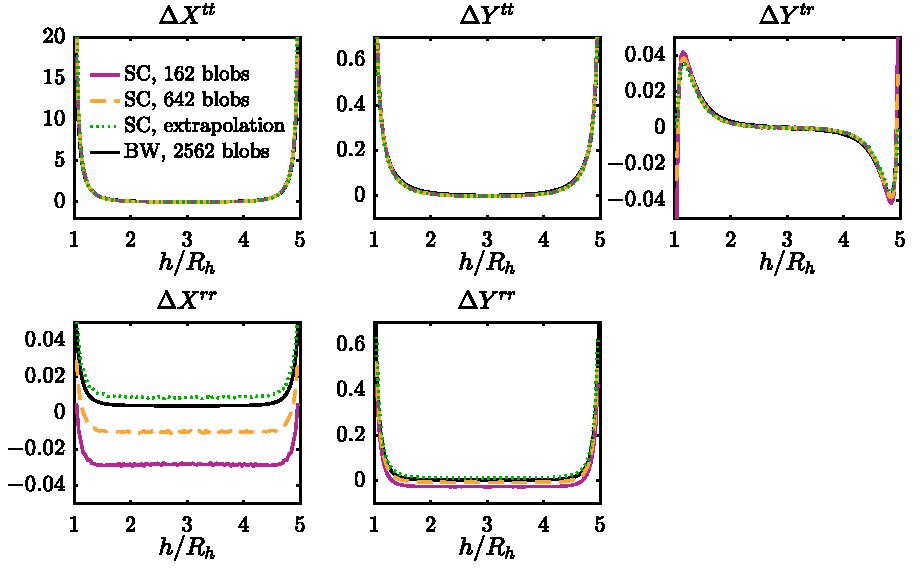
\includegraphics{rollers_dR_coef.pdf}};
\newcommand{\Width}{1.75in};
\newcommand{\x}{6.12in};
\newcommand{\y}{0.25in};
\node[anchor=south east,inner sep=0pt] (B) at (\x,\y) {\resizebox{\Width}{!}{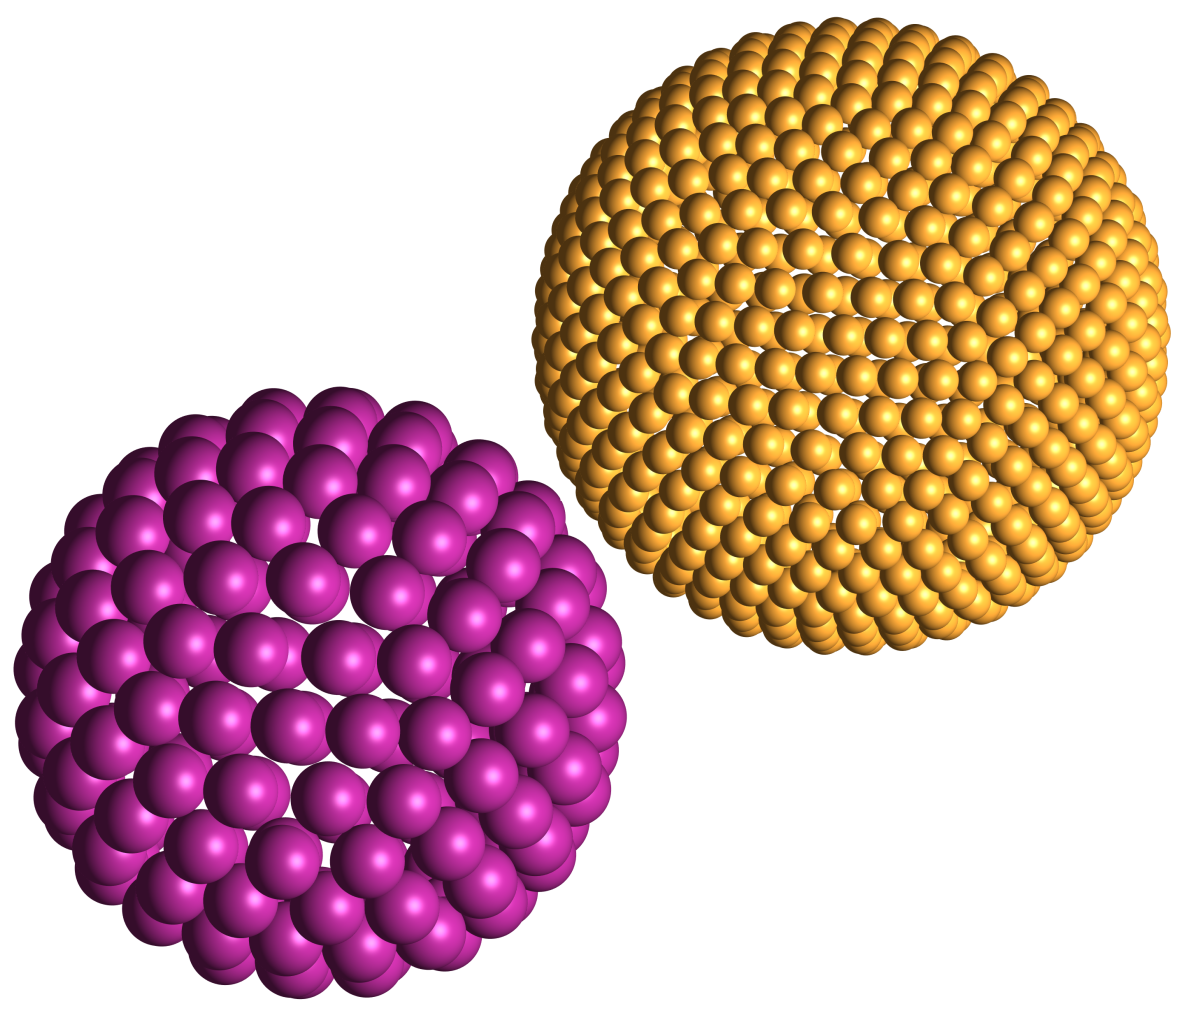
\includegraphics{rollers_dR_coef_inset.png}}};

\definecolor{mygoldcolor}{rgb}{0.9883,0.6523,0.2114};
\definecolor{mypurpcolor}{rgb}{0.6928,0.1651,0.5645};

\node[anchor=north west] at ($(B.north west)+(0.1in,0)$) {\large{\textcolor{mygoldcolor}{\textbf{$642$ blobs}}}};
\node[anchor=south east] at ($(B.south east)+(-0.1in,0)$) {\large{\textcolor{mypurpcolor}{\textbf{$162$ blobs}}}};

\end{tikzpicture}

\end{document}
